
\chapter{Intermediate Representations}
\begin{figure}[ht]
	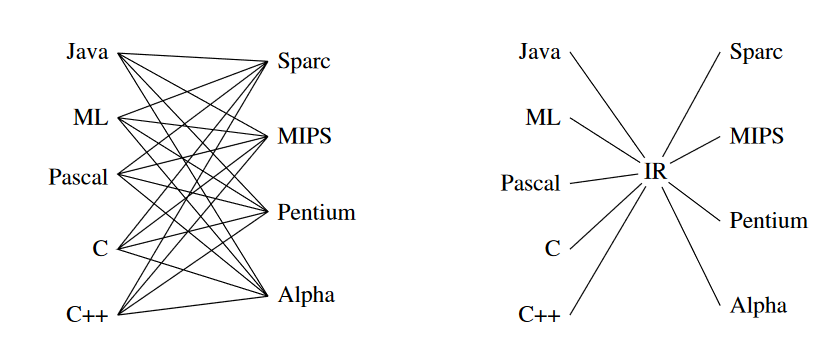
\includegraphics[width=\textwidth]{intermediate_representations}
	\caption{Compilers voor vijf talen en vier architecturen: 
		(links) geen IR, (rechts) met IR.}
	\label{fig:intermediate_representations}
\end{figure}
Een goede IR moet:
\begin{itemize}
	\item makkelijk te produceren zijn door de compiler frontend
	\item makkelijk zijn om er echte assembler van te genereren
	\item duidelijke, eenvoudige betekenis hebben
\end{itemize}

Een IR-tree is een eenvoudige abstractie van machine-instructies. Het lijkt heel goed op een Abstract Syntax Tree maar is taal-onafhankelijk en werkt met temporaries in plaats van variabelen.

Typen van expressies (\texttt{T\_exp}):
\begin{itemize}
	\item \texttt{CONST(i)}: integer constante $i$
	\item \texttt{NAME(n)}: assembly label $n$
	\item \texttt{TEMP(t)}: virtueel register $t$
	\item \texttt{BINOP(o, $e_1$, $e_2$)}: $e_1 o e_2$ met $o = +, -, *, /, ...$. Hier wordt $e_1$ altijd eerst geëvalueerd.
	\item \texttt{MEM(e)}: De inhoud van $w$ bytes op $e$ schrijven of lezen.
	\item \texttt{CALL(f, $l_1, ..., l_n$)}: roep $f$ op met argumenten $l_i$. De volgorde van de argumenten is van belang.
	\item \texttt{ESEQ(s, e)}: evalueer $s$ voor neveneffecten, dan $e$ als resultaat.
\end{itemize}

Typen van statements:
\begin{itemize}
	\item \texttt{MOVE(TEMP t, e)}: evalueer $e$ en wijs toe aan temp $t$.
	\item \texttt{MOVE(MEM($e_1$), $e_2$)}: evalueer $e_1$ tot adres $a$, evalueer $e_2$ en schijf het in de $w$ bytes vanaf $a$.
	\item \texttt{EXP(e)}: evalueer $e$ en negeer het resultaat.
	\item \texttt{JUMP(e, labs)}: evalueer $e$ tot een adres en spring er naar. 
	\item \texttt{CJUMP(e ...)}:
	\item \texttt{SEQ($s_1$, $s_2$)}: sequentie van statements 
\end{itemize}

Er is geen 1-op-1 mapping van \texttt{A\_EXP} naar \texttt{T\_EXP}.

\QA{Waarom staan er NULL pointers?}{We weten nog niet naar waar we moeten springen. Er moeten labels inkomen, maar we kennen ze nog niet. Voorlopig dienen die dus als placeholders.}

patchlist bevat de labels (in gelinkte lijst vorm) in geval van true en geval van false. De constructor bevat het hele pad in de IR tree naar het lege veld vanaf de root van het statement ($s_1$ in voorbeeld). Als de waarde 0 of 1 in \texttt{flag} moet komen kan de expressie geconverteerd worden naar een andere expressies. Program 7.3: steek 1 in temporary, als we false uitkomen wordt 0 in temporary gestoken. De doPatch functie kent een label toe aan een bepaald veld in de boom.

\subsection{Omzetting enkelvoudige veranderlijken}

$+$ symbool is dereference operator


l-values:
\begin{itemize}
	\item kan links in een toewijzing voorkomen
	\item verwijst naar een locatie
\end{itemize}

r-values:
\begin{itemize}
	\item kan enkel rechts in een toewijzing voorkomen
	\item verwijst impliciet naar een waarde
\end{itemize}

scalar:
\begin{itemize}
	\item Waarde die slechts één geheugenwoord bevat.
\end{itemize}



